\documentclass[11pt]{scrartcl}
\usepackage{amsmath, amssymb, amscd, amsthm, amsfonts}
\usepackage{graphicx}
\usepackage{hyperref}
\usepackage[english]{babel}
\usepackage[utf8]{inputenc}
\usepackage{xcolor}
% \usepackage{algorithm}
\usepackage{cancel}
\usepackage{csquotes}
\usepackage{bm}
\usepackage{appendix}
\usepackage{url}
\usepackage{parskip}
\usepackage{float}
\usepackage{subfigure}
\usepackage{graphicx}
\usepackage{wrapfig}
\usepackage[square,numbers]{natbib}
\usepackage{caption}
\usepackage{amsmath}
\usepackage{hyperref}

\bibliographystyle{unsrt}

\oddsidemargin 0pt
\evensidemargin 0pt
\marginparwidth 40pt
\marginparsep 10pt
\topmargin -60pt
\headsep 0pt
\textheight 9.5in
\textwidth 6.65in
\linespread{1.0}

\DeclareMathOperator{\enc}{\textbf{enc}}
\DeclareMathOperator{\gen}{\textbf{gen}}
\DeclareMathOperator{\cost}{\textbf{cost}}

\title{Toxic Comment Classification}
\subtitle{NLP Project - Master IASD}
\author{Xavier GEFFRIER, Léonard de LA SEIGLIÈRE}
\date{April 2022}

\begin{document}

\maketitle

The code of this project can be found \href{https://github.com/leonarddls/NLP_projet}{HERE} : \begin{verbatim} https://github.com/leonarddls/NLP_projet \end{verbatim}


\section{Problem Presentation}

\subsection{Objective}

Our objective in this project is to train a model to detect and label "toxic" text comments. This is semantic analysis. For each comment, written by a human, we want to apply from 0 to 6 labels, the labels being \textit{toxic}, \textit{severe\_toxic}, \textit{obscene}, \textit{threat}, \textit{insult}, \textit{identity\_hate}.

\subsection{Data presentation}

Data is composed of English text comments posted on Wikipedia, in  the "Discussion" section of Wikipedia pages. It is a very interesting dataset. First it is huge (around 160K rows), moreover it is free and without any copyright, and most importantly it has been labelled by humans, allowing simple supervised learning.

Most comments are shorts (less than 100 words) as we can see on Figure \ref{fig:sizes}. The majority has no toxic label (Figure \ref{fig:all-labels}), and among the classified ones, some labels are much more frequent (Figure \ref{fig:labels}). Note that one comment can be labeled for multiple toxic behaviors, for instance be classified simultaneously as \textit{insult} and \textit{identity\_hate}.

\begin{figure}[H]
    \centering
    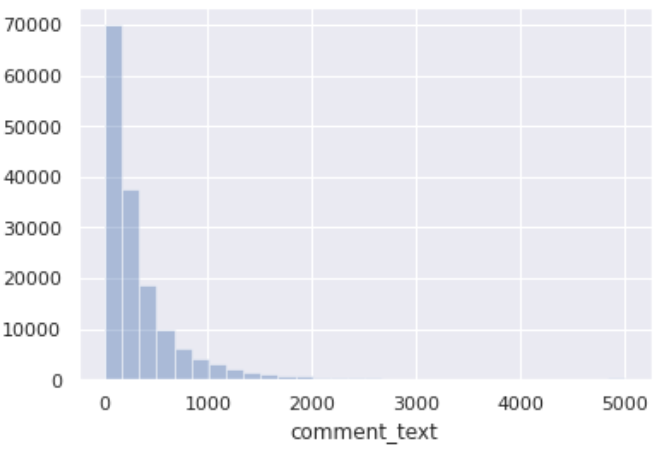
\includegraphics[width=10cm]{img/size.PNG}
    \caption{Histogram showing repartition of comments by size.}
    \label{fig:sizes}
\end{figure}

\begin{figure}[H]
    \centering
    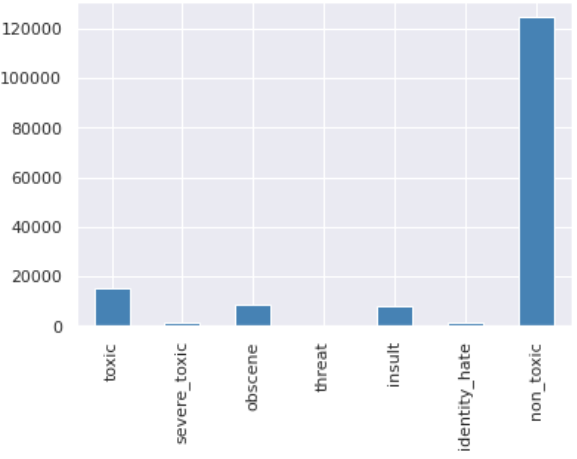
\includegraphics[width=10cm]{img/all_labels_frequency.PNG}
    \caption{Frequency of each label among comments including non-toxic comments.}
    \label{fig:all-labels}
\end{figure}

\begin{figure}[H]
    \centering
    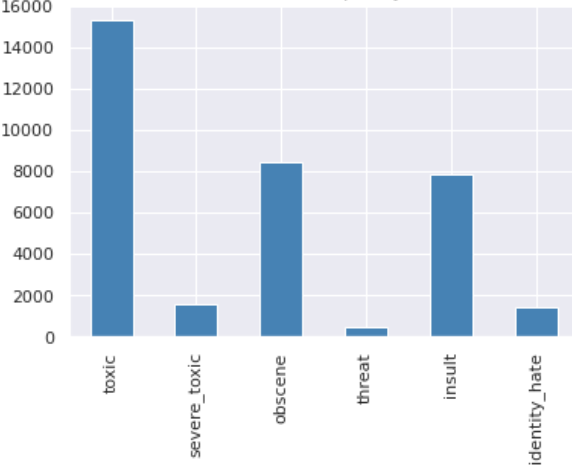
\includegraphics[width=10cm]{img/labels_frequency.PNG}
    \caption{Frequency of each label excluding non-toxic comments.}
    \label{fig:labels}
\end{figure}



\subsection{Plan and evaluation}

We will try three different methods and compare them by using the AUC-ROC (Area Under the Curve - Receiver Operating Characteristics), which seemed a better metric than F1-score that we first planned to use.

F1-score is useful to evaluate classification models with 2 classes or more, and is defined as the harmonic mean of precision and recall. It is especially used when data is unbalanced like in disease or fraud detection, and in our case, that is why we first thought it could be a good metric.

AUC-ROC is also designed for classification problem, and also use the false positive rate (FPR) and true positive rate (TPR). ROC is a probability curve, plotted with TPR against the FPR (see Figure \ref{fig:aoc}). The area under the curve, AUC, gives us an idea of how model is good to separate data. The best possible value is 1: no false positive. AUC-ROC is good too when dealing with unbalanced classes.


\begin{figure}[h]
    \centering
    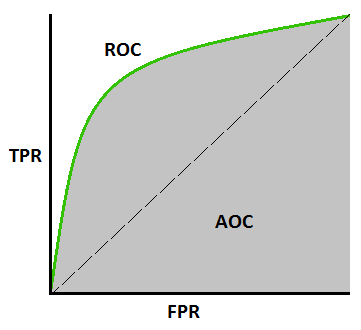
\includegraphics[width=9cm]{img/auc.png}
    \caption{AOC-ROC curve \cite{narkhede_2018}}
    \label{fig:aoc}
\end{figure}


The main difference between the two is that the F1 score takes predicted classes as an input, and AUC-ROC predicted scores (or probability). So when we want to evaluate a model like a neural network, which can output probabilities, AUC is a better option, since F1-score would require that we set a threshold to actually classify data.

Our first method will be a T\textbf{F-IDF associated with a Decision Tree classifier}, which is a basic method that will give us some standard score to evaluate the others. Then we will train and use a \textbf{LSTM} neural network. Then, a \textbf{BERT} model.

\section{The Three methods}

\subsection{TF-IDF and Decision Tree}

\subsubsection{About TF-IDF}
TF-IDF stands for Text Frequency - Inverse Document Frequency. It is a very basic way to have an idea of the "importance" of each word in a text, by just computing its frequency, that is to say the number of occurrences divided by the text length, and compare it to the frequency in the whole document (i.e. in other texts).

We then use a Decision Tree on the output of the TF-IDF to classify a text and already have a small classifier.

\subsubsection{Our work}

TODO: Leonard ?

\subsection{LSTM}

\subsubsection{About LSTM}

Long-short term memory (LSTM) is a very well-known architecture of recurrent neural networks (RNN), proposed by Hochreiter et al. (1997) \cite{hochreiter1997long}. Their intention was trying to analyse sequence of data, while dealing with the vanishing gradient problem, that affected previously existing RNNs. The long-term gradients which were propagated could tend to zero and vanish, or to infinity and explode, due to finite-precision numbers of machines. LSTM networks can still have this exploding gradient problem, but vanishing is partially solved thaks to a distinction between the hidden state (similar to the output of a simple RNN cell) and the cell state, useful to keep track of long-term memory.

Since we learned in class how an LSTM work, we will not give more details and directly say how we used it.

\subsubsection{Our work}

TODO : Leonard ?

\subsection{BERT}

\subsubsection{About Transformers and BERT}
The Transformer is a kind of neural network architecture that has been created by Vaswani et al. (2017)\cite{vaswani2017attention} initially to perform translation. Until that, recurrent neural networks like LSTM were used but they come with a few drawbacks: \label{lstm-drawbacks}
\begin{itemize}
    \item First, they are slow to train. Since each word has to be passed sequentially, it is not possible to parallelize the learning and to accelerate it by just adding more GPUs.
    \item Then, they can only treat limited sequences at once, and can "forget" the beginning of a long paragraph when parsing the end of it.
    \item For each word, they do not take surrounding context into account, but only sequence up to this word. Bidirectionnal LSTM attempt to fix that by reading the sequences backward and forward (see Figure \ref{fig:bilstm}) but they only manage to concatenate both informations, and fail to treat them as one more compelte information.
\end{itemize}

\begin{figure}[H]
    \centering
    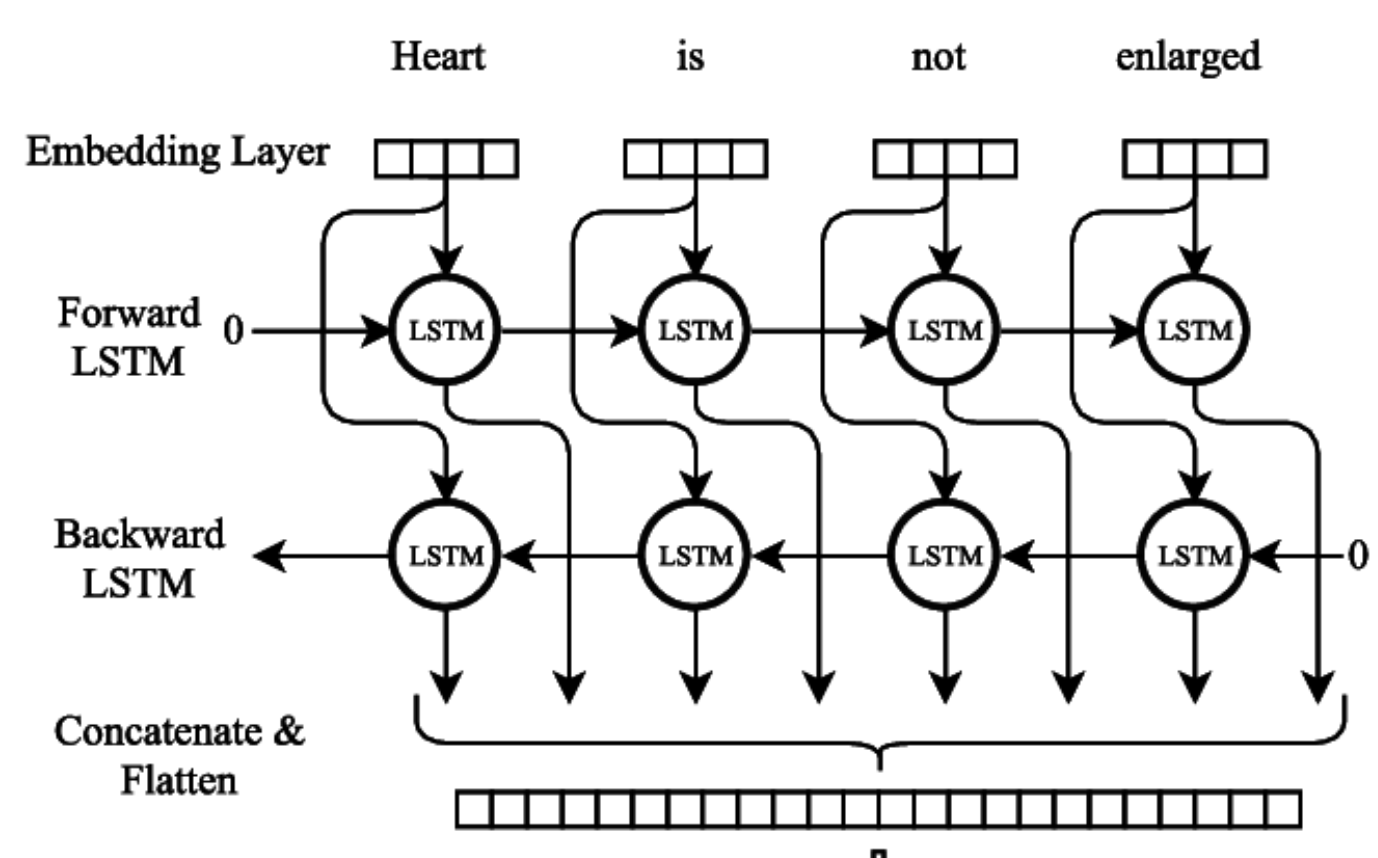
\includegraphics[width=12cm]{img/BiLSTM.png}
    \caption{Schema of a bidirectional LSTM: both directions are taken into account, but in a parallel way with concatenation at the end, and not as one global information.}
    \label{fig:bilstm}
\end{figure}

Transformer are designed to fix these flaws with three main changes:
\begin{enumerate}
    \item \textbf{Positional encoding:} each word is enriched with its position (index) as an input, so that model can have information about the order of the sequence.
    \item \textbf{Attention:} the words that we must pay attention to in the source language when translating a word on the destination language, an idea proposed by Bahdanau et al. (2014)\cite{bahdanau2014neural} that uses learning over examples.
    \item \textbf{Self-attention:} the internal representation of a language, by using context of words.
\end{enumerate}

The Transformer consists in an encoder and a decoder (see Figure \ref{fig:transformer}). The encoder create embeddings from input words simultaneously, and the decoder use them and the current output translated words to continue translation, one word at a time.

This separation in tasks is useful. The encoder learns what the source language is, what the context is. The decoder learns how words of one language relate to the other ones. By interesting ourselves only on the decoder and stacking some of them, we obtain a GPT. In the same way, if we stack the encoders, we get BERT.

BERT stands for a Bidirectional Encoder Representation from Transformers. BERT can be used for translation, as well as text summarization or, what is important to us, sentiment analysis. 

\begin{figure}[]
    \centering
    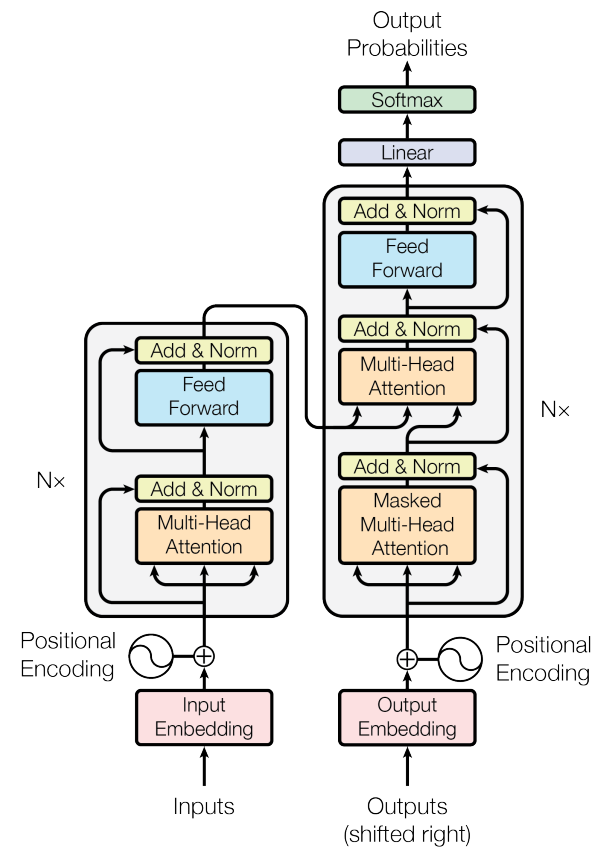
\includegraphics[height=10cm]{img/Transformer.PNG}
    \caption{Schema of a Transformer from the original paper of Vaswani et al.\cite{vaswani2017attention}}
    \label{fig:transformer}
\end{figure}

\subsubsection{Our work}

TODO : Leonard ?

\section{Results}


\begin{table}[H]
\begin{center}
\begin{tabular}{| r | c |}
\hline
Method & AUC (validation data) \\ \hline \hline
Decision tree & 0 \\ \hline
LSTM & 0.9809 \\ \hline
BERT & 0.9828 \\ \hline
\end{tabular}
\end{center}
\caption{\label{tab:result-table}Results obtained on validation data for each method.}
\end{table}

These results are not exactly what we expected. We thought that TF-IDF + DT would be the less precise classifier, and it is. However, LSTM and BERT are almost indistinguishable, while we figured out that BERT would outperform LSTM. In fact, the difference in their score is so tiny that in some of our trys, it was LSTM that was first: we can not conclude that one of them is better for this particular problem.

How can we explain this? First, it is quite hard to train layers added to a pre-trained BERT model. The forward pass takes a lot of time, simply because the number of parameteres is huge. So we may have not trained enough our model, due to this constraint. But this is unlikely: the AUC was not growing anymore.

A more likely hypothesis is that both models perform well and that we can not really expect any model to perform better. The drawbacks of LSTM that we mentioned in section \ref{lstm-drawbacks} are not problematic in this dataset. Most comments are short enough for LSTM memory. A simple sequential view of the words is enough to determine their toxicity, even if it is not a real context observation like in BERT. If the hypothesis is right, then LSTM may be preferred, because it required less computation power x time to train it.

\bibliographystyle{alpha}
\bibliography{references}
\appendix

\end{document}
